\chapter{Spektrale Methoden\label{chapter:klima}}
\lhead{Spektrale Methoden}
\begin{refsection}
\chapterauthor{Peter Nötzli}

\rhead{}
\section{Einleitung
\label{klima:einleitung}}

\begin{figure}
\centering
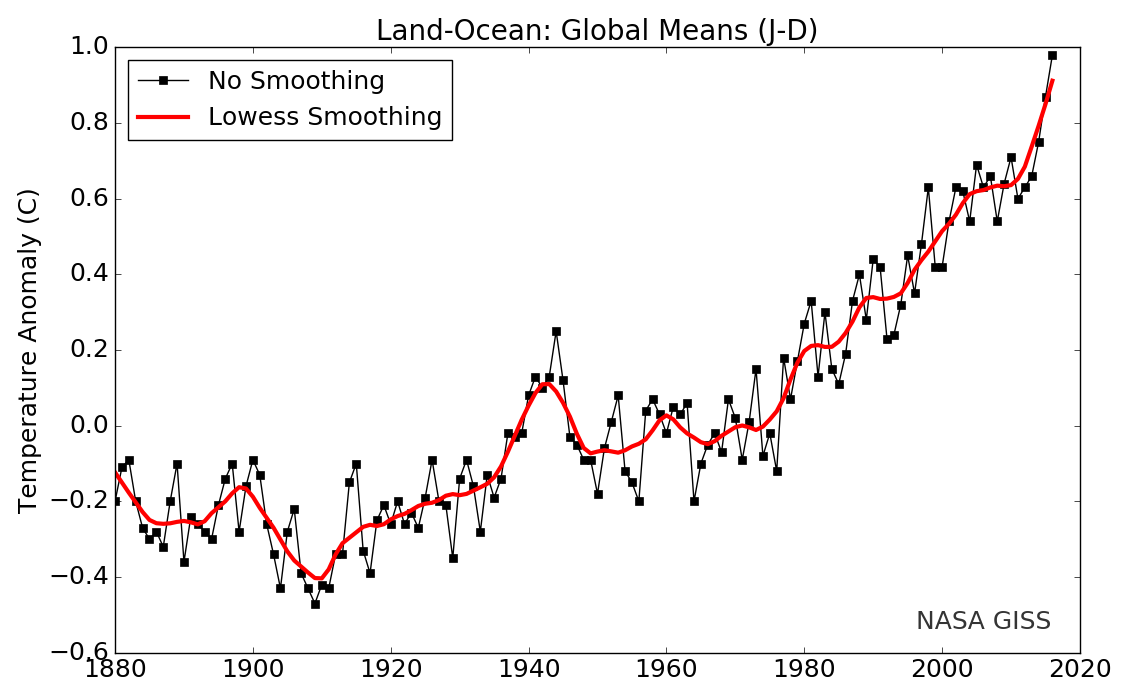
\includegraphics[width=\hsize]{klima/nasa_giss.png}
\caption{Grafik der globalen Jahresmitteltemperaturen seit 1880. Quelle: National Aeronautics and Space Administration Goddard Institute for Space Studies kurz NASA GISS \url{https://data.giss.nasa.gov/gistemp/graphs/customize.html}.
\label{klima:einleitung:nasa}}
\end{figure}

Die Klimaerwärmung schreitet voran, gleichzeitig, oder gerade deswegen kommen in der Gesellschaft dazu immer mehr Fragen auf. Gibt es eine Klimaerwärmung? Wie entwickelt sich diese? Was bedeutet dies für uns? Betrifft es mich überhaupt? Die erste und wohl einfachste Frage vorweg, ja es gibt die Klimaerwärmung. Dies ist deutlich zu erkennnen wenn wir die globale Temperaturentwicklung seit 1880 bis heute betrachten, schaue dazu Abbildung~\ref{klima:einleitung:nasa}. Diese Frage ist deshalb einfach zu beantworten, da diese nach einem Ereignis Frägt welches bereits, oder zumindest teilweise, in der Vergangeheit liegt. Die Auswirkungen dieses Ereignisses und wie weit es sich noch entwicklen wird sind Dinge welche in der Zukunft liegen. Somit kann für die restlichen Fragen und auch viele der nicht gestellten Fragen keine pauschale Antwort gegeben werden. Obwohl eine Tendenz der roten Linie in Abbildung~\ref{klima:einleitung:nasa} erkennbar ist, dies von Hand und mit ein bisschen Gefühl weiter zu führen kann wohl nicht richtig sein, da es sämtliche Faktoren welche einen Einfluss auf das Klima haben ignoriert. Da wir dennoch gerne wissen wollen welche Einflüsse welche Auswirkungen haben und wir auch nicht warten möchten bis es bereits zu spät ist, müssen wir auf Klimamodelle zurückgreifen. Wie so ein Klimamodell ausschauen könnte und wie es aufgebaut sein kann möchte ich in diesem Kapitel aufzeigen.



\section{Geschichte der Numerischen Strömungsmechanik
\label{section:klima:geschichte}}
Die numerische Strömungsmechanik, heute auch als CFD bekannt (Computational Fluid Dynamics) ist eine etablierte Methode um verschiedenste Problemstellungen der Strömungsmechanik approximativ mit numerischen Modellen zu lösen. Die Validierung der Methoden erfolgt durch den Vergleich mit quantitativen Experimenten.


\subsection{Entstehung der Wettervorhersagen
\label{subsection:klima:wetter}}
Am Anfgang war das Wetter. Dann kam der Mensch und wollte wissen, wie das Wetter in Zukunft sein wird. Dies aus verschiedensten Gründen so wollen wir heute gerne wissen, welches Wetter am Wochenende ist, damit wir bereits anfangs Woche einen Ausflug organisieren können. Bedeutung hatten Wettervorhersagen, früher wie heute, so kann eine Wettervorhersage wesentlichen Einfluss auf das Ernteglück haben. So entstanden schon früh sogenannte Bauernregeln, diese gingen meist davon aus dass sich das Wetter aufgrund Wetterereignissen an bestimmten Tagen in eine gewisse Richtung entwickeln. Die Korrektheit solcher Aussagen sind wohl eher Zufälle als korrekte Vorhersagen, so sind es eher die ähnlichen Wetterverhältnisse der jeweiligen Jahreszeit welchee solch eine Regel von Zeit zu Zeit als korrekt erscheinen lässt. Jedoch waren verschiedenste Naturphänomene bereits bekannt, als Beispiel die Silberdiestel, auch als Wetterdiestel bekannt, welche seine Blütenblätter bei erhöhter Luftfeuchtigkeit aufrollt und so vor nahendem Regen warnen kann.
1660 erkannte Otto von Guericke erstmals den Zusammenhang zwischen abfallendem Luftdruck und dem aufziehen eines Unwetters.
Anfangs des 19. Jahrhunderts entstanden in Europa die ersten Wetterstationen, es waren jedoch noch keine Wettervorhersagen mölich. Dies aus dem einfachen Grund, da sich das Wetter schneller in eine nahende Statt bewegen konnte als man die Daten dort hinbringen hätte können.
1835 konnte mit dem aufkommen der Telegrafie dieses Problem gelöst werden, erstmals waren einfache Prognosen möglich. Diese reichten oft nur einzelne Tage in die Zukunft, waren lokal begrenzt. Die Genauigkeit dieser ist nicht mit heutigen Massstäben vergleichbar.
Vilhelm Bjerknes (1862-1951) war der erste, welcher erkannte dass die Problemstellung der Wettervorhesage sich aus Physik und Mathematik zusammen setzt. Im wesentlichen stellte er fest, dass für die Berechnung der Strömung der Atmosphäre genaue Kenntnisse der Grundgesetze und der Anfangsbestimmungen notwendig und ausreichend für eine Wettervorhersage sind.


\subsection{Lewis Fry Richardson
\label{subsection:klima:richardson}}

\begin{figure}
\centering
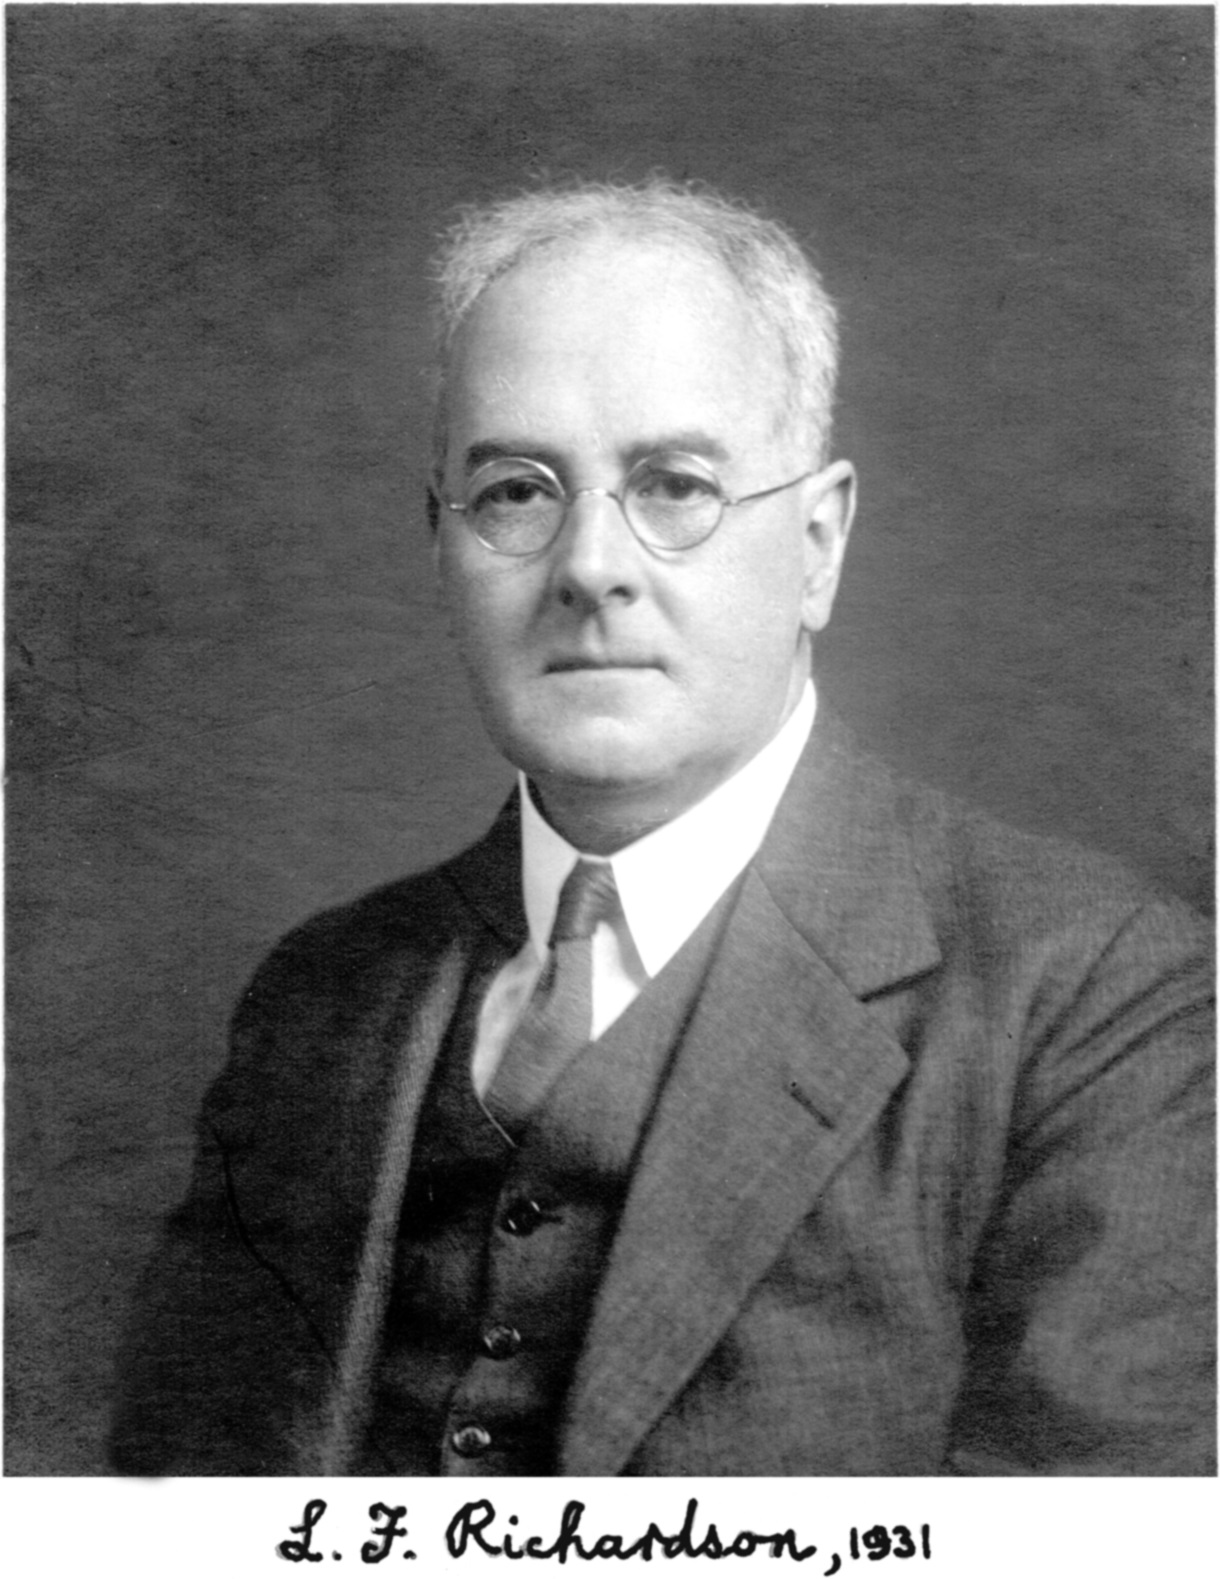
\includegraphics{klima/richardson.jpg}
\caption{Lewis Fry Richardson \cite{klima:biography}
\label{klima:geschichte:richardson}}
\end{figure}

Lewis Fry Richardson (1881-1953) Abbildung~\ref{klima:geschichte:richardson} veröffentlichte 1922 seine Arbeit mit dem Titel {\em Weather Prediction by Numerical Process}, in welcher er die erste numerische Wettervorhersage tätigte.
Für seine Berechnungen, die er um 1917 durchführte, verwendete er Druck- und Temperatur-Daten verschiedenster Stationen in Europa. Er legte für seine Berechnung ein Gitter über Europa, dieses hatte eine Breite von 2°89' und eine Länge von 1°80'Höhe, und 5 vertikale Layer. Dies entspricht in etwa einer Abmessung von 130km mal 200km je Feld und umfasst ingesamt etwa 150 Punkte an welchen die Drucktendenz berechnet werden sollte. Er verwendete dabei die horizontalen Impulserhaltungsgleichungen, die ideale Gasgleichung und die Kontinuitätsgleichung (diese haben wir bereits im Kapitel \ref{subsection{Energie-Impuls-Erhaltung}} \nameref{subsection{Energie-Impuls-Erhaltung}} auf der Seite \pageref{subsection{Energie-Impuls-Erhaltung}} angeschaut). Die Vorhersage für 24 Stunden bedeutete dabei einen Rechenaufwand von 3 Monaten.
Im wesentlichen basierte die Berechnung auf einer Unterteilung in die einzelnen Zellen welche jeweils mit 7 Werten befüllt waren. Dies waren der Luftdruck, Temperatur, Dichte, Luftfeuchtigkeit und den Volumenströmen richtung Norden, Osten und Aufwärts.
Die erste Berechnung von Richardson lieferte dann auch ein Resultat, welches einen Druckabfall von 145mbar in 6h voraussagte. Eine solch grosse Veränderung ist absolut unrealistisch und nichteimal im Zentrum eines Sturmtiefes möglich. Das Problem war, dass die Daten des Boden-Drucks, welche als Anfangsbedinungen verwendet wurden, fehler enthielten. Diese Fehler führten dazu, dass sich während der numerischen Prozedur die Werte aufschaukelten und somit zu hohen Drucktendenzen führten. (Eine Berechnung aufgrund der selben Beobachtungsdaten, die jedoch zu Beginn gefiltert werden, führt mit Richardson's Algorithmus zu plausiblen Vorhersagen, 3.2 mbar in 6h) \cite{klima:stocker}).
Dies zeigt exemplarisch wie heikel die Anfangsbedingungen von Wetter- und Klimamodellen sich auf das Ergebniss auswirken können. Jedoch hätten selbst die besten Initialisierungswerte zu einer Instabilität geführt und eine Resultat für grosse Vorhersagezeiten verunmöglicht.
Erst durch die Verfügbarkeit erster Computer in den 40er Jahren wurde Richardsons Arbeit zur  Wettervorhersage praktikabel und wurde gegen Ende des 2. Weltkriegs als taktisches Mittel eingesetzt.

\begin{figure}
\centering
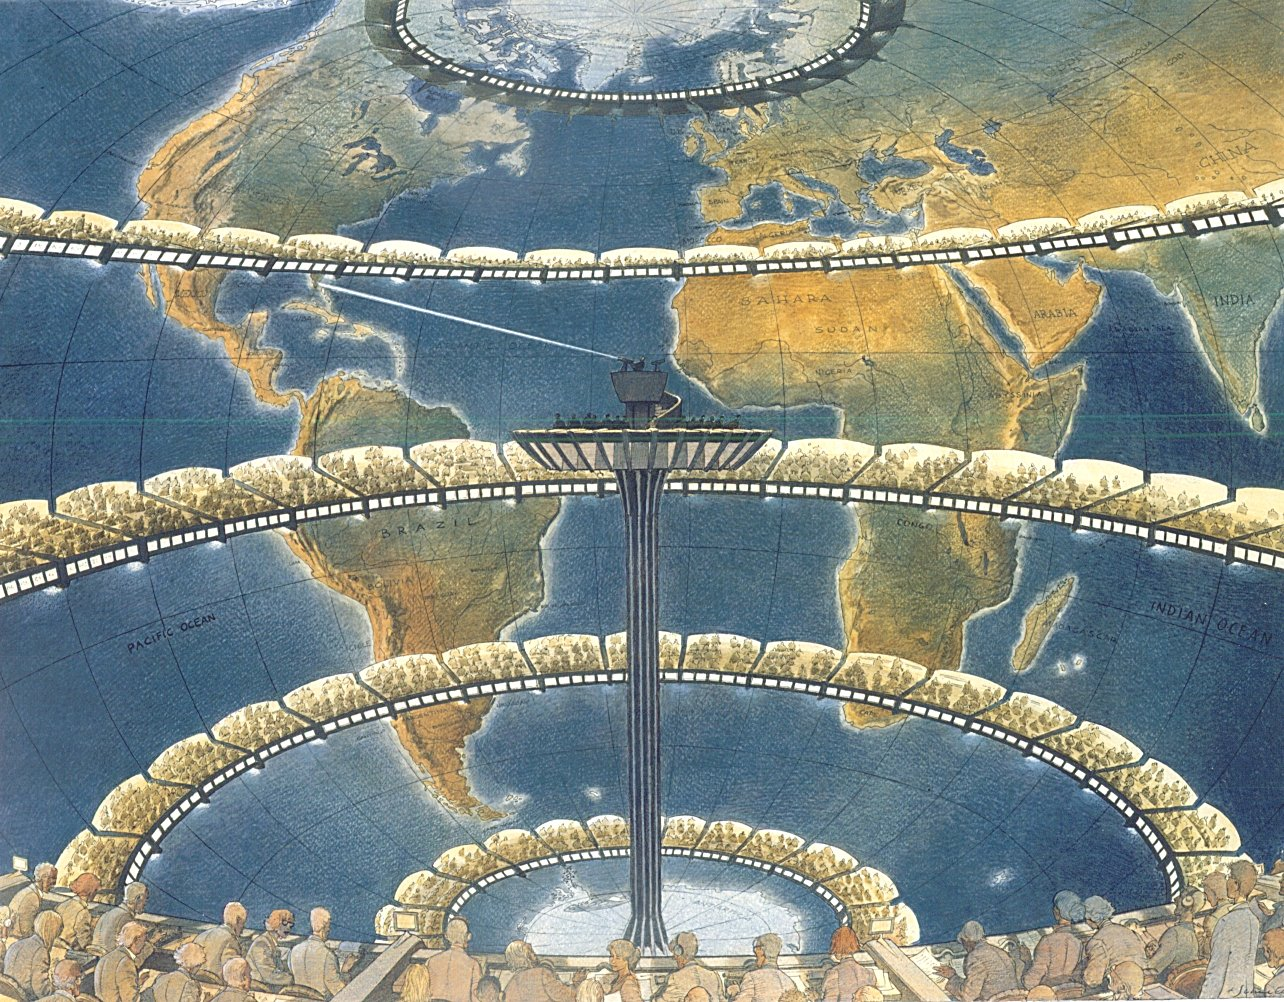
\includegraphics{klima/64000.jpg}
\caption{Interpretation eines Künstlers von Richardsons Vorhersage Fabrik \cite{klima:biography}
\label{klima:geschichte:richardson}}
\end{figure}

Richardson äusserte in seiner Arbeit die Idee einer Vorhersage Fabrik in welcher er mit 64'000 Rechnern (damit waren damals noch Menschen gemeint), welche gleichzeitig Berechnungen durchführten und zum weiterrechnen jeweils die Werte ihrer Nachbarzellen übernehmen sollten, das Wetter für den ganzen Planeten berechnen könnte. Diese Idee wurde vom Künstler François Schuiten in der Abbildung~\ref{klima:geschichte:richardson} versinnbildlicht.
Zudem äusserte Richardson einen weiteren Traum, von welchem wir heute wissen das es möglich ist.
\begin{quote}
Perhaps some day in the dim future it will be possible to advance the computations faster than the weather advances....
\end{quote}

\subsection{Wettervorhersagen in der Schweiz
\label{section:klima:wettervorhersagen}}
Meteo Schweiz und 7 private Weterdienste
System
Genauigkeit (Zeitschritt)

Weshalb (Berge, Täler)
Schwierigkeiten von Unwetter und Gewitter erkennung
COSMO
Ensemble Rechnungen (leicht variierende Initialwerte, dies gibt bei der Auswertung die Möglichkeit die korrekte Prognose mit einer höheren Wahrscheinlichkeit zu prophezeien


\subsection{Klimavorhersagen
\label{subsection:klima:entstehung}}
Unterschied Wetter/Klima

Enflussrössen und Kipppunkte im Klimasystem(Albedoeffekt, auftauen Permafrost)

 










\section{Spektrale Methoden
\label{section:klima:spektrale}}
Im gegensatz zur klassischen Strömungsmechanik wählen die Spektralen Methoden einen globalen Ansatz. Hierbei wird nicht mit Druck, Temperatur und weiteren Werten gerechnet sondern mit spektralen koeffizienten welche sich mit einer Fast Fourrier Transformation wieder zurück.

Vorteile

sphärisch harmonische Analyse zum heruasfinden der a's unb b's

Vergleich mit klassischen Methoden

Einflüsse wie Rückkopllungseffekte





\subsection{Beispiel mit Wärmeleitung
\label{subsection:klima:beispiel}}
Ein einfachere Variante, mit der wärmeleitegleichung auf einem Kreis, befindet sich als Übungsaufgabe am Ende des Kapitels \ref{skript:chapter:kugelfunktionen} \nameref{skript:chapter:kugelfunktionen} auf der Seite \pageref{skript:1101:pdgl}.

Benötigt wird die allgemeine Wärmeleitegleichung:
\begin{equation}
\frac{\partial T}{\partial t} = \Delta T  \lambda
\label{klima:bsp:pdgl}
\end{equation}



%Achtung, ab hier ist einiges zusammen kopiert und angepasst. Unbedingt überarbeiten! Kopie aus Übungsaufgabe und auf Kugel angepasst
%%%%%%%%%%%%%%%%%%%%%%%%%%%%%%%%%%%%%%%%%%%%%%%%%%%%%%%%%%%%%%%%%%%%%%%

Fourier-Reihe auf einer Kugel
\begin{equation}
T(\vartheta ,\varphi ,t)
=
a_{00}(t) + \sum_{l=1}^\infty\sum_{m=0}^l \bigl( a_{lm}(t)Y_{lm}(\vartheta ,\varphi)+b_{lm}(t)Z_{lm}(\vartheta ,\varphi)\bigr)
\end{equation}

Laplace-Operator für Kugelfunktion
\begin{equation}
\Delta f = \frac{1}{r^2} \frac{\partial}{\partial r} \left( r^2 \,\frac{\partial f}{\partial r} \right) + \frac{1}{r^2 \sin \vartheta} \frac{\partial}{\partial \vartheta} \left(\sin\vartheta \, \frac{\partial f}{\partial \vartheta} \right) + \frac{1}{r^2 \sin^2\vartheta} \frac{\partial^2 f}{\partial \varphi^2}
\end{equation}

Dieser Schritt ist mir absolut nicht klar, woher weis ich dass? Und wenn es gegeben ist, woher? Oder hat das garnichts mit dem Laplace-Operator zu tun und ich verwechsle hier etwas?
\begin{equation}
\Delta Y_{lm}=-l(l+1)Y_{lm}
\end{equation}

$Y$ können mithilfer der Basisfunktion Formel \ref{skript:kugelfunktione:Y} auf Seite \pageref{skript:kugelfunktione:Y}





Wir müssen die Fourier-Reihe~\eqref{skript:1101:ansatz} für
$T(\vartheta ,\varphi ,t)$ in die Differentialgleichung~\eqref{klima:bsp:pdgl}
einsetzen.
Dazu berechnen wir erst die Ableitungen nach $t$:
\begin{align*}
\frac{\partial T}{\partial t} &=
\dot{a}_{00}(t)+\sum_{l=1}^\infty\sum_{m=0}^l \bigl( \dot{a}_{lm}(t)Y_{lm}(\vartheta ,\varphi)+\dot{b}_{lm}(t)Z_{lm}(\vartheta ,\varphi)\bigr)
\\
\Delta T(\vartheta ,\varphi ,t) &=
\phi^c - \sum_{l=1}^\infty\sum_{m=0}^l \bigl( a_{lm}(t)l(l+1)Y_{lm}(\vartheta ,\varphi)+b_{lm}(t)l(l+1)Z_{lm}(\vartheta ,\varphi)\bigr)
\end{align*}
Die Differentialgleichung verlangt, dass diese beiden Terme übereinstimmen,
also folgen die gewöhnlichen Differentialgleichungen

Woher kommt dieses $\phi^c$ überhaupt?
\begin{align*}
\dot a_{00}(t)&=\phi^c
\\
\dot a_{lm}(t)&=l(l+1)a_{lm}(t)&
\dot b_{lm}(t)&=l(l+1)b_{lm}(t)
\end{align*}
Man beachte, dass die erste Gleichung als Speziallfall in der ersten
Gleichung der zweiten Zeile enthalten ist.
\begin{align*}
a_{lm} &=Ce^{-l(l+1)t}&
b_{lm} &=Ce^{-l(l+1)t}
\end{align*}

$a_{00}$ könnte wie folgt aussehen
\begin{align*}
a_{00}(t)&=ct+T_0
\end{align*}









\printbibliography[heading=subbibliography]
\end{refsection}